\title{Economic Time Series HW2}
\author{Daeyoung Lim}

\documentclass[answers]{exam}
\usepackage[left=3cm,right=3cm,top=3.5cm,bottom=2cm]{geometry}
\usepackage{amssymb,amsmath,amsfonts,amsthm}
\usepackage{mathtools}
\usepackage{graphicx}
\usepackage{kotex}
\usepackage[utf8]{inputenc}
\usepackage[T1]{fontenc}
\usepackage{lmodern}
% \usepackage{enumerate}
\usepackage{listings}
\usepackage{courier}
\usepackage{cancel}
\usepackage{array}
\usepackage{courier}
\usepackage{booktabs}
\usepackage{titlesec}
\usepackage[shortlabels]{enumitem}
\usepackage{setspace}
\usepackage{newtxtext}
\usepackage[lite,nofontinfo,zswash,straightbraces]{mtpro2}
\usepackage{empheq}
\usepackage{tikz}
\usepackage{listings}
\usepackage{titlesec}

% \usepackage[toc,page]{appendix}

\setlength{\heavyrulewidth}{1.5pt}
\setlength{\abovetopsep}{4pt}

\DeclarePairedDelimiter{\ceil}{\lceil}{\rceil}
\newcommand\encircle[1]{%
  \tikz[baseline=(X.base)] 
    \node (X) [draw, shape=circle, inner sep=0] {\strut #1};}
 
% Command "alignedbox{}{}" for a box within an align environment
% Source: http://www.latex-community.org/forum/viewtopic.php?f=46&t=8144
\newlength\dlf  % Define a new measure, dlf
\newcommand\alignedbox[2]{
% Argument #1 = before & if there were no box (lhs)
% Argument #2 = after & if there were no box (rhs)
&  % Alignment sign of the line
{
\settowidth\dlf{$\displaystyle #1$}  
    % The width of \dlf is the width of the lhs, with a displaystyle font
\addtolength\dlf{\fboxsep+\fboxrule}  
    % Add to it the distance to the box, and the width of the line of the box     ㅊ
\hspace{-\dlf}  
    % Move everything dlf units to the left, so that & #1 #2 is aligned under #1 & #2
\boxed{#1 #2}
    % Put a box around lhs and rhs
}
}
\setcounter{secnumdepth}{4}
\lstset{
         basicstyle=\footnotesize\ttfamily, % Standardschrift
         %numbers=left,               % Ort der Zeilennummern
         numberstyle=\tiny,          % Stil der Zeilennummern
         %stepnumber=2,               % Abstand zwischen den Zeilennummern
         numbersep=5pt,              % Abstand der Nummern zum Text
         tabsize=2,                  % Groesse von Tabs
         extendedchars=true,         %
         breaklines=true,            % Zeilen werden Umgebrochen
         keywordstyle=\color{red},
            frame=b,         
 %        keywordstyle=[1]\textbf,    % Stil der Keywords
 %        keywordstyle=[2]\textbf,    %
 %        keywordstyle=[3]\textbf,    %
 %        keywordstyle=[4]\textbf,   \sqrt{\sqrt{}} %
         stringstyle=\color{white}\ttfamily, % Farbe der String
         showspaces=false,           % Leerzeichen anzeigen ?
         showtabs=false,             % Tabs anzeigen ?
         xleftmargin=17pt,
         framexleftmargin=17pt,
         framexrightmargin=5pt,
         framexbottommargin=4pt,
         %backgroundcolor=\color{lightgray},
         showstringspaces=false      % Leerzeichen in Strings anzeigen ?        
 }
 \lstloadlanguages{% Check Dokumentation for further languages ...
         %[Visual]Basic
         %Pascal
         %C
         %C++
         %XML
         %HTML
         Java
 }
    %\DeclareCaptionFont{blue}{\color{blue}} 

\definecolor{myblue}{RGB}{72, 165, 226}
\definecolor{myorange}{RGB}{222, 141, 8}
\titleformat{\paragraph}
{\normalfont\normalsize\bfseries}{\theparagraph}{1em}{}
\titlespacing*{\paragraph}
{0pt}{3.25ex plus 1ex minus .2ex}{1.5ex plus .2ex}
\setlength{\heavyrulewidth}{1.5pt}
\setlength{\abovetopsep}{4pt}
\setlength{\parindent}{0mm}
\linespread{1.3}
\DeclareMathOperator{\sech}{sech}
\DeclareMathOperator{\csch}{csch}
\DeclareMathOperator*{\argmin}{\arg\!\min}
\DeclareMathOperator{\Tr}{Tr}

\newcommand{\bs}{\boldsymbol}
\newcommand{\opn}{\operatorname}
%%%%%%%%%%%%%%%%%%%%%%%%%%%%%%%%%%%%%%%%%%%%%%%%%%%%%%%
% % We use newtheorem to define theorem-like structures
% %
% % Here are some common ones. . .
%%%%%%%%%%%%%%%%%%%%%%%%%%%%%%%%%%%%%%%%%%%%%%%%%%%%%%%
% \newtheorem{theorem}{Theorem}
% \newtheorem{lemma}{Lemma}
% \newtheorem{proposition}{Proposition}
% \newtheorem{scolium}{Scolium}   %% And a not so common one.
% \newtheorem{definition}{Definition}
% \newenvironment{proof}{{\sc Proof:}}{~\hfill QED}
% \newenvironment{AMS}{}{}
% \newenvironment{keywords}{}{}
%%%%%%%%%%%%%%%%%%%%%%%%%%%%%%%%%%%%%%%%%%%%%%%%%%%%%%%
% %   The first thanks indicates your affiliation
% %
% %  Just the name here.
% %
% % Your mailing address goes at the end.
% %
% % \thanks is also how you indicate grant support
% %
%%%%%%%%%%%%%%%%%%%%%%%%%%%%%%%%%%%%%%%%%%%%%%%%%%%%%%%


\begin{document}
\setstretch{1.5} %줄간격 조정
\newpage
\firstpageheader{}{}{\bf\large Daeyoung Lim \\ Economic Time Series \\ Fall Semester, 2016}
\runningheader{Daeyoung Lim}{Economic Time Series}{Fall Semester, 2016}
Download CD.txt, GDP.txt, CPI.txt from the course webpage. CD.txt contains quarterly CD (91 days) rates from 1991.Q1 to 2013.Q4; GDP.txt contains GDP growth rates (year-on-year) from 1971.Q1 to 2013.Q4; and CPI.txt contains consumer price index from 1965.Q1 to 2013.Q4.
\begin{questions}
    \question
    Plot interest rates (CD rates), growth rates (GDP growth rates), and inflation rates from 1991.Q1 to 2013.Q4 in a figure with 3 by 1 format. Inflation rates are obtained as $100\times (\log \text{CPI}_{t}-\log \text{CPI}_{t-4})$.
    \begin{solution}
        The plot looks as follows.
        \centering
        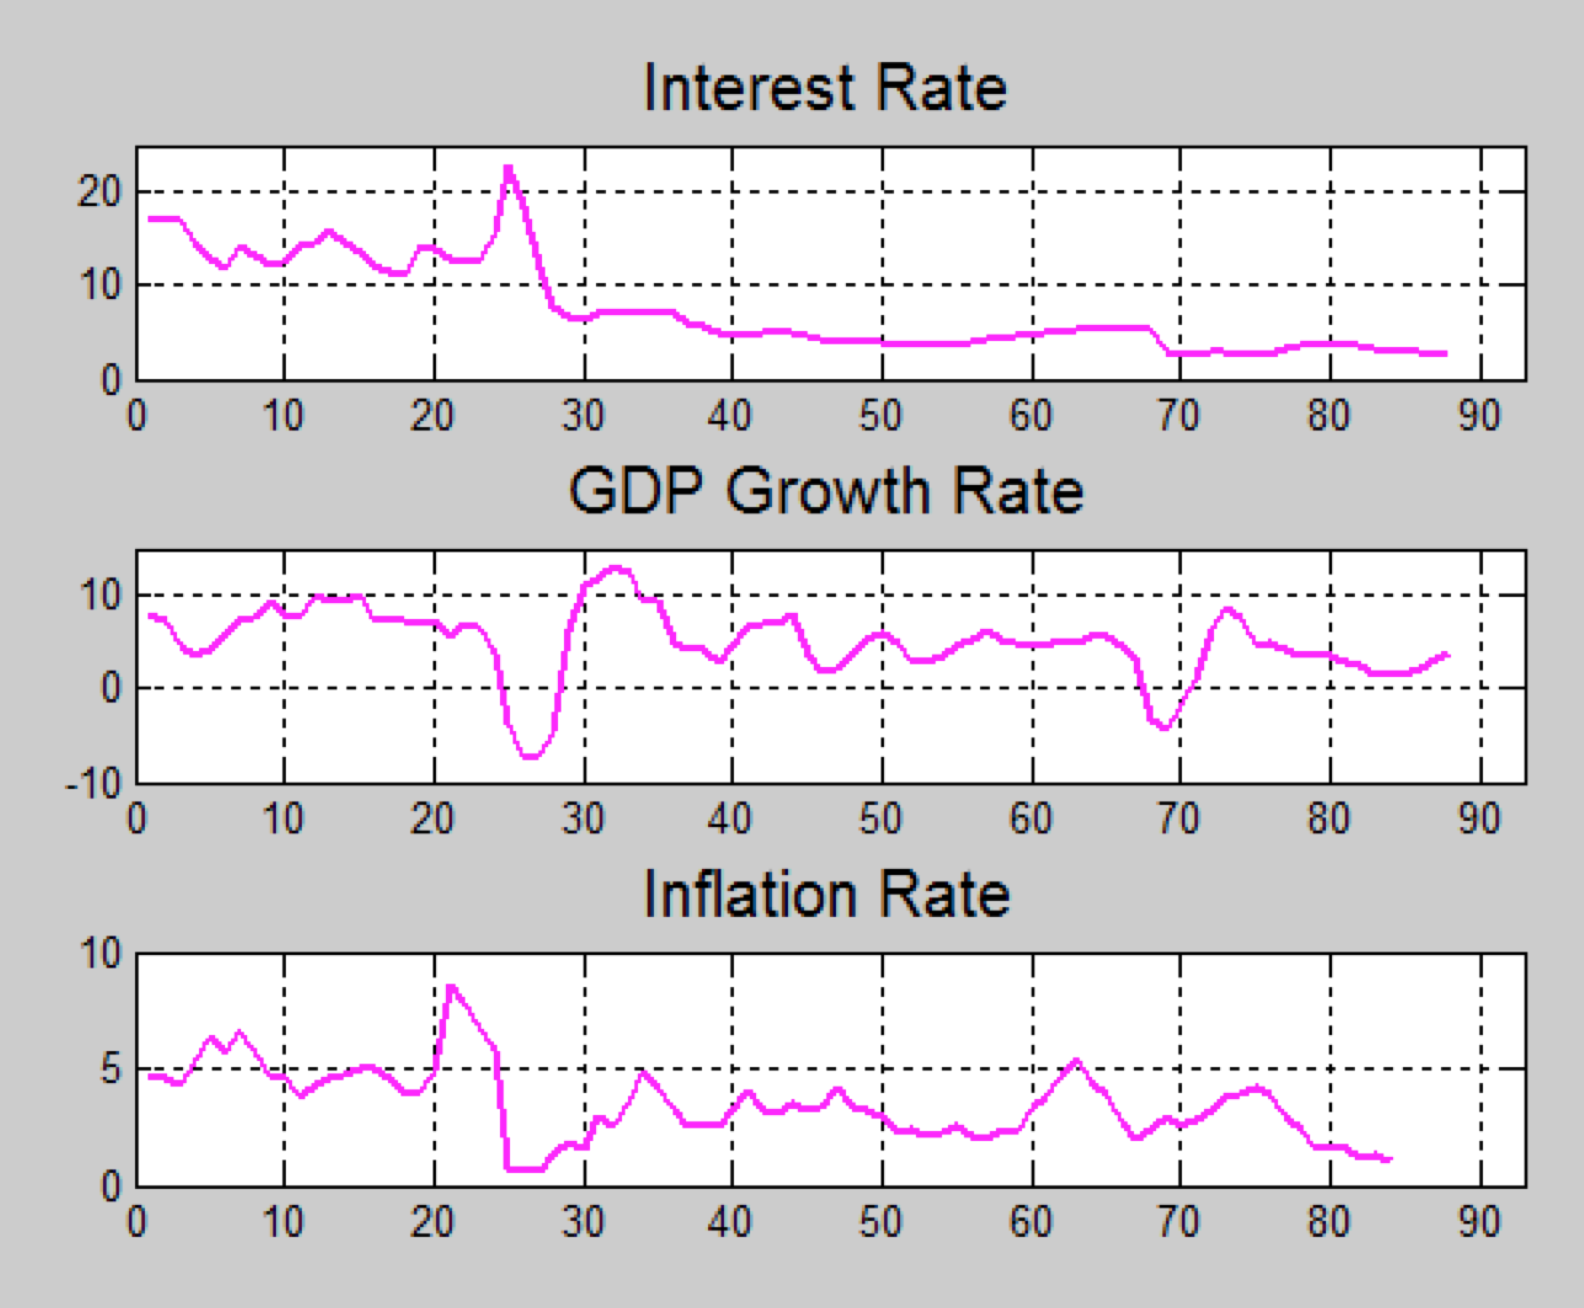
\includegraphics[scale=0.5]{Problem1.png}
    \end{solution}
    \newpage
    \question Compute the autocorrelation functions of the three variables and report the results as the following figure.
    \begin{solution}
        The plot is as follows.
        \centering
        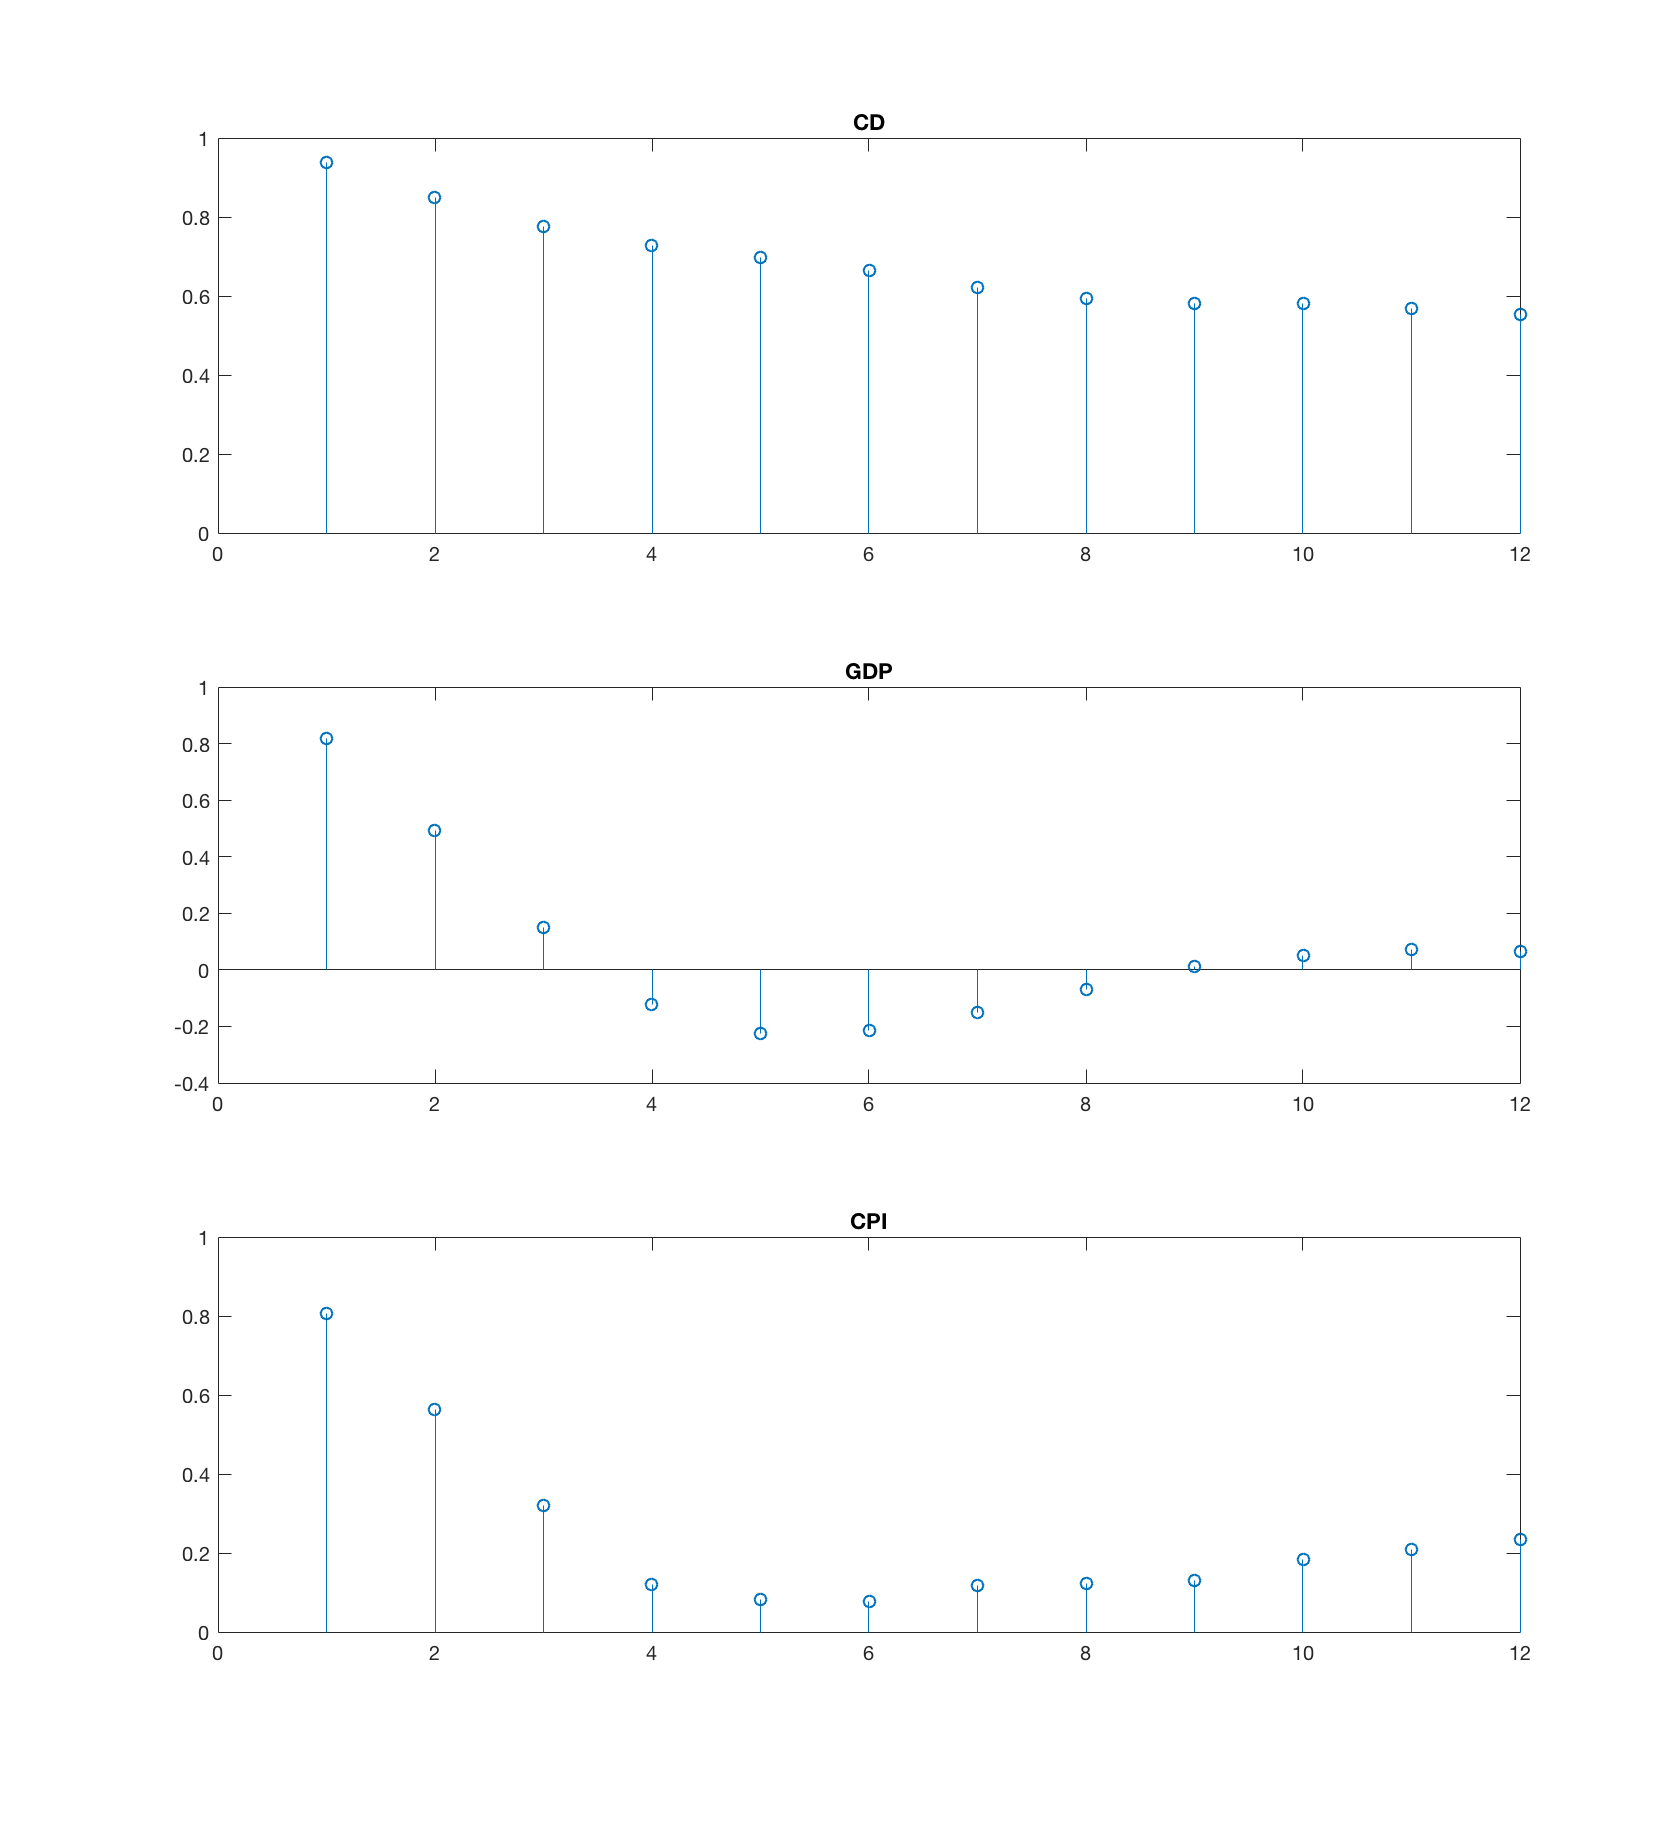
\includegraphics[scale=0.2]{Problem2.png}
    \end{solution}
    \question
    Test the hypothesis of white noise for each of the three variables, $H_{0}:\rho(1)=\cdots = \rho (\tau_{\max})=0$, where $\tau_{\max}=6$. Report the p-values.
    \begin{solution}
        P-values are all zero. Therefore, we can conclude that the interest rate, GDP growth rate, and inflation rate are not white noise processes.
    \end{solution}
    \question
    Suppose that each of the three variables is an ARMA(2,1) process,
    \begin{align}
        X_{t} &= \mu+a_{1}X_{t-1}+a_{2}X_{t-2}+e_{t}+b_{1}e_{t-1}\\
        e_{t}&\sim \mathcal{N}\left(0,\sigma^{2}\right)
    \end{align}
    Estimate $\left(a_{1},a_{2},b_{1},\sigma^{2}\right)$ for each of the three variables using \texttt{chap2\_Estimation.m} in the lecture note.
    \begin{solution}
    \begin{itemize}
        \item Inflation rate
        % \begin{table}[!htbp]
        % \begin{table}
          \begin{center}
          \begin{tabular}{*5c}
            \toprule
            $\mu$ & $a_{1}$ & $a_{2}$ & $b_{1}$ & $\sigma^{2}$ \\
            \midrule
            $0.5402$ & $-0.0831$ & $0.9895$ & $0.3406$ & $1.7917$\\
            \bottomrule
          \end{tabular}
          \end{center}
        % \end{table}
        \item GDP growth rate
        \begin{center}
          \begin{tabular}{*5c}
            \toprule
            $\mu$ & $a_{1}$ & $a_{2}$ & $b_{1}$ & $\sigma^{2}$ \\
            \midrule
            $1.2697$ & $-0.6726$ & $1.4113$ & $-0.1978$ & $3.2555$\\
            \bottomrule
          \end{tabular}
          \end{center}
        \item Inflation rate
        \begin{center}
          \begin{tabular}{*5c}
            \toprule
            $\mu$ & $a_{1}$ & $a_{2}$ & $b_{1}$ & $\sigma^{2}$ \\
            \midrule
            $1.0489$ & $0.4700$ & $0.2485$ & $0.9734$ & $0.6697$\\
            \bottomrule
          \end{tabular}
          \end{center}
    \end{itemize}
    \end{solution}
    \question
    Now, consider a VAR system consisting of inflation rates, growth rates, and interest rates.
    \begin{enumerate}[(a)]
        \item Test if one variable Granger-causes another variable. Note that there are 6 permutations in total.
        \item Plot impulse response functions and forecast error variance decompositions up to 16 horizons. In doing so, identify structural parameters using short-run restrictions by assuming that the causal chain holds in the order of inflation rates, growth rates, and inflation rates. Interpret your results.
        \item Repeat (b) with long-run restrictions. How do your results change? Explain main differences.
    \end{enumerate}
    \begin{solution}
        \begin{enumerate}[(a)]
            \item Testing if there is a Granger causality between the three variables, the results are as follows.
            \begin{itemize}
                \item $H_{0}:$ GDP growth rate does not Granger-cause the interest rate.
                \begin{center}
                  \begin{tabular}{*1c}
                    \toprule
                    $p$-value\\
                    \midrule
                    0.0006\\
                    \bottomrule
                  \end{tabular}
                \end{center}
                \item $H_{0}: $ The inflation rate does not Granger-cause the interest rate.
                \begin{center}
                  \begin{tabular}{*1c}
                    \toprule
                    $p$-value\\
                    \midrule
                    0.9514\\
                    \bottomrule
                  \end{tabular}
                \end{center}
                \item $H_{0}: $ The interest rate does not Granger-cause the GDP growth rate.
                \begin{center}
                  \begin{tabular}{*1c}
                    \toprule
                    $p$-value\\
                    \midrule
                    0.0.1712\\
                    \bottomrule
                  \end{tabular}
                \end{center}
                \item $H_{0}: $ The inflation rate does not Granger-cause the GDP growth rate.
                \begin{center}
                  \begin{tabular}{*1c}
                    \toprule
                    $p$-value\\
                    \midrule
                    0.2523\\
                    \bottomrule
                  \end{tabular}
                \end{center}
                \item $H_{0}: $ The interest rate does not Granger-cause the inflation rate.
                \begin{center}
                  \begin{tabular}{*1c}
                    \toprule
                    $p$-value\\
                    \midrule
                    0.0490\\
                    \bottomrule
                  \end{tabular}
                \end{center}
                \item $H_{0}: $ The GDP growth rate does not Granger-cause the inflation rate.
                \begin{center}
                  \begin{tabular}{*1c}
                    \toprule
                    $p$-value\\
                    \midrule
                    0.0538\\
                    \bottomrule
                  \end{tabular}
                \end{center}
            \end{itemize}
            \item The plot is as follows.\par
            \begin{center}
            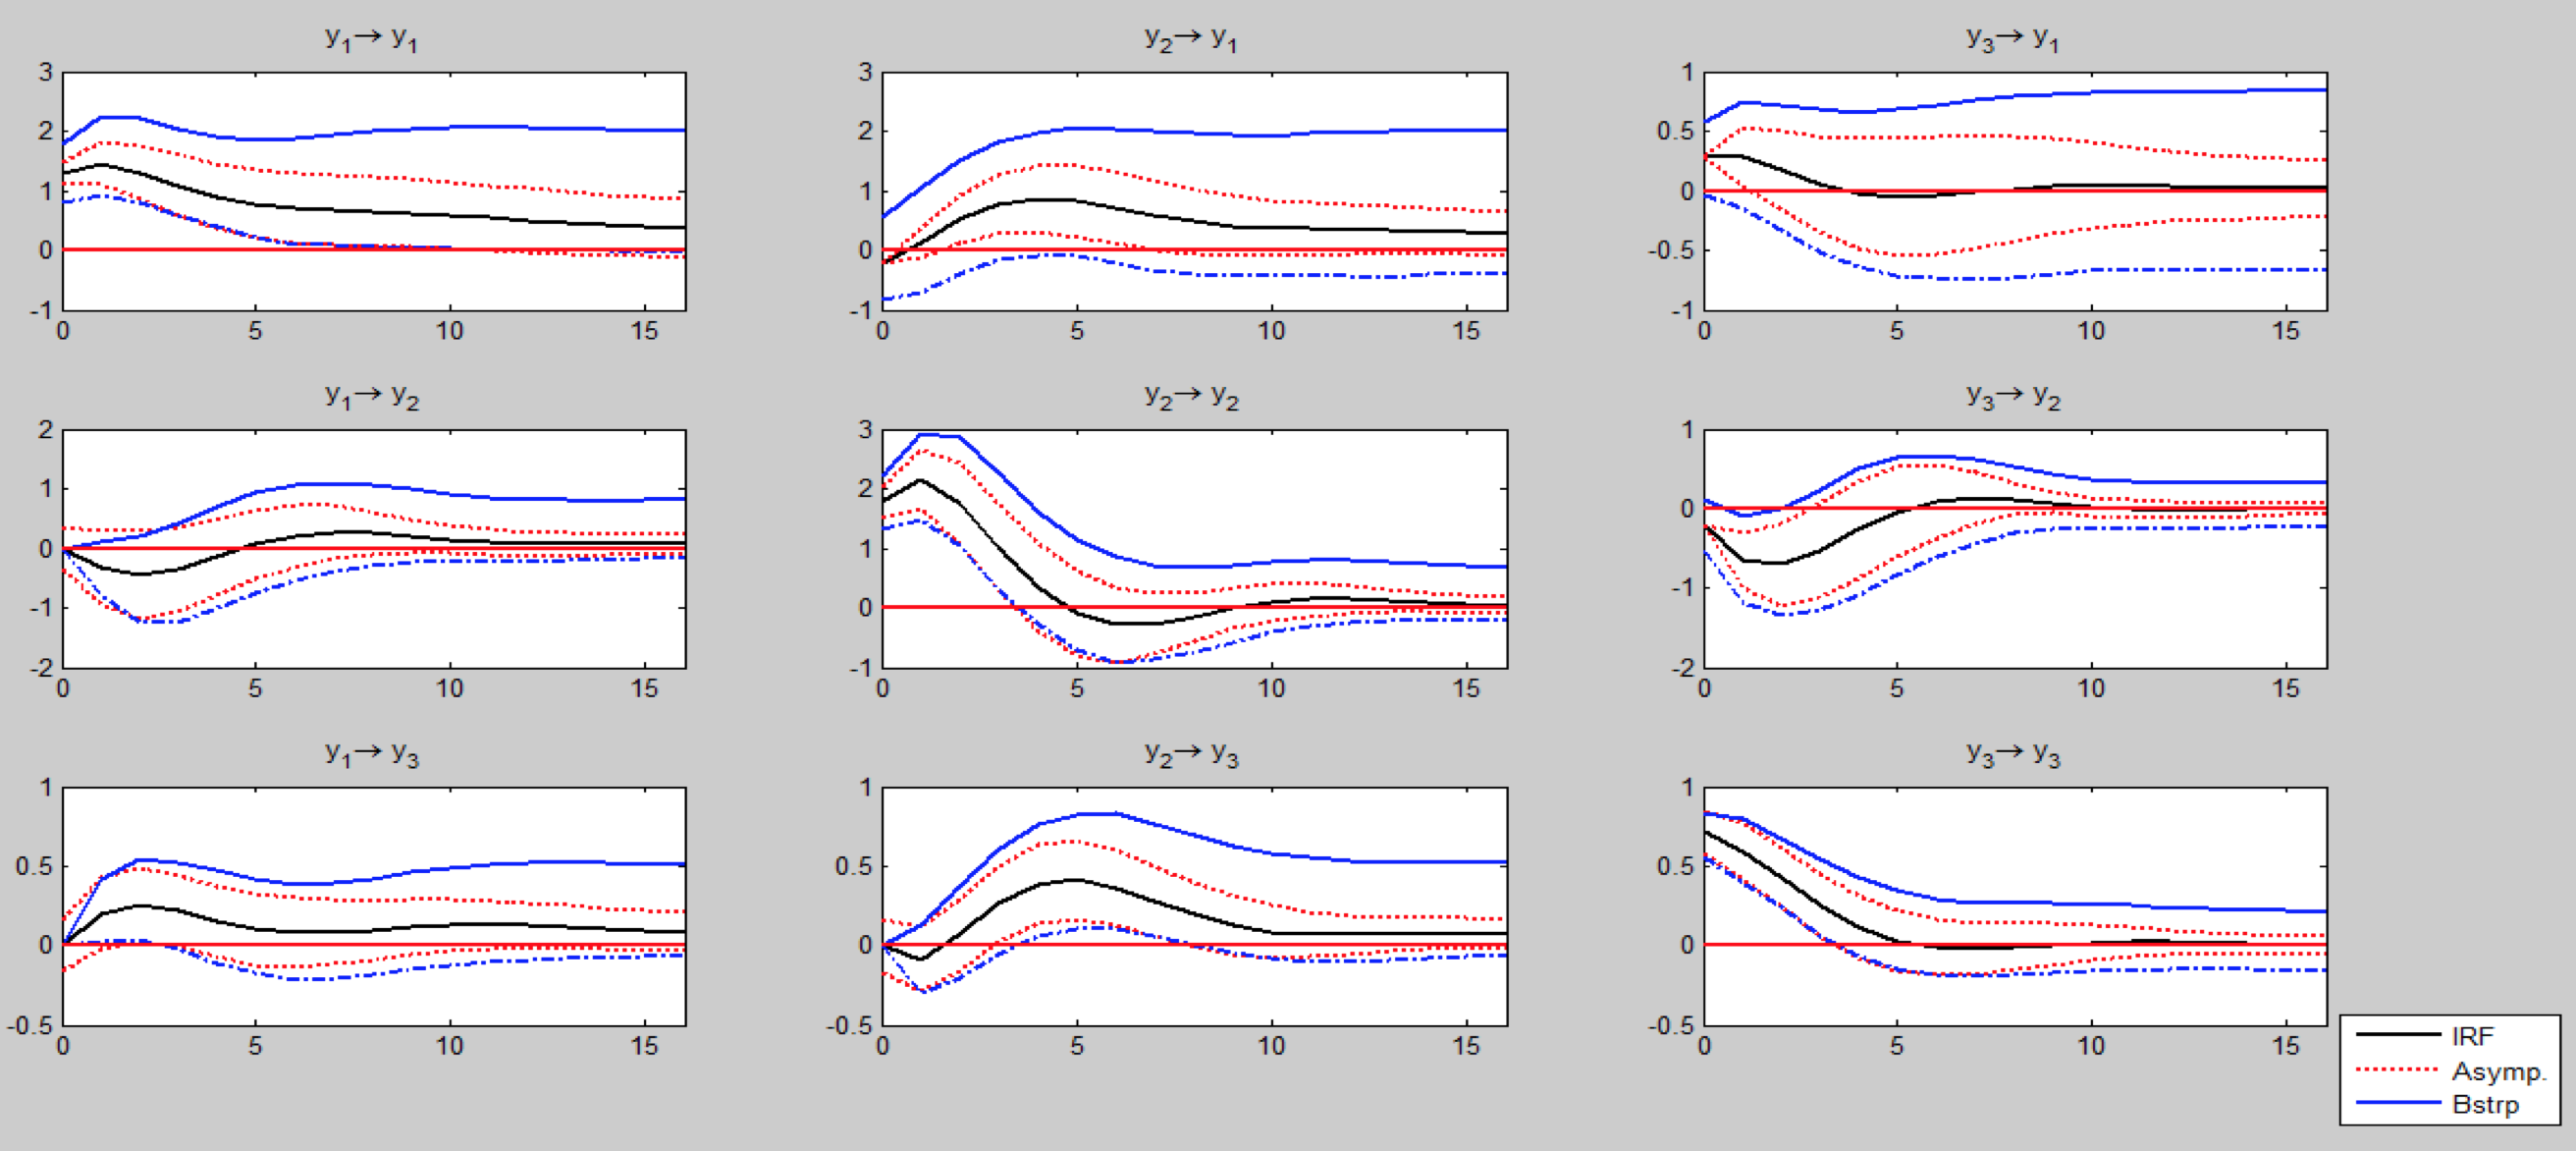
\includegraphics[scale=0.25]{Problem3.png}
            \end{center}
            \par
            Accordingly to common knowledge, it is known that the interest rate and the growth rate have negative correlation and so do the interest rate and the inflation rate. On the other hand, the inflation rate and the growth rate are known to be correlated positively. However, when we look at the above plots, the $(2,3)^{\text{th}}$ plot demonstrates that the inflation rate and the growth rate are moving in the opposite direction. Likewise, $(3,1)^{\text{th}}$ plot tells us that the inflation rate increases---rather than decrease---as the error of the interest rate increases. These results that are in conflict with our common sense showed up because we have omitted some relevant variables from the regression.\par
            Moving on to the forecast error variance decompositions, below are the plots.
            \begin{center}
            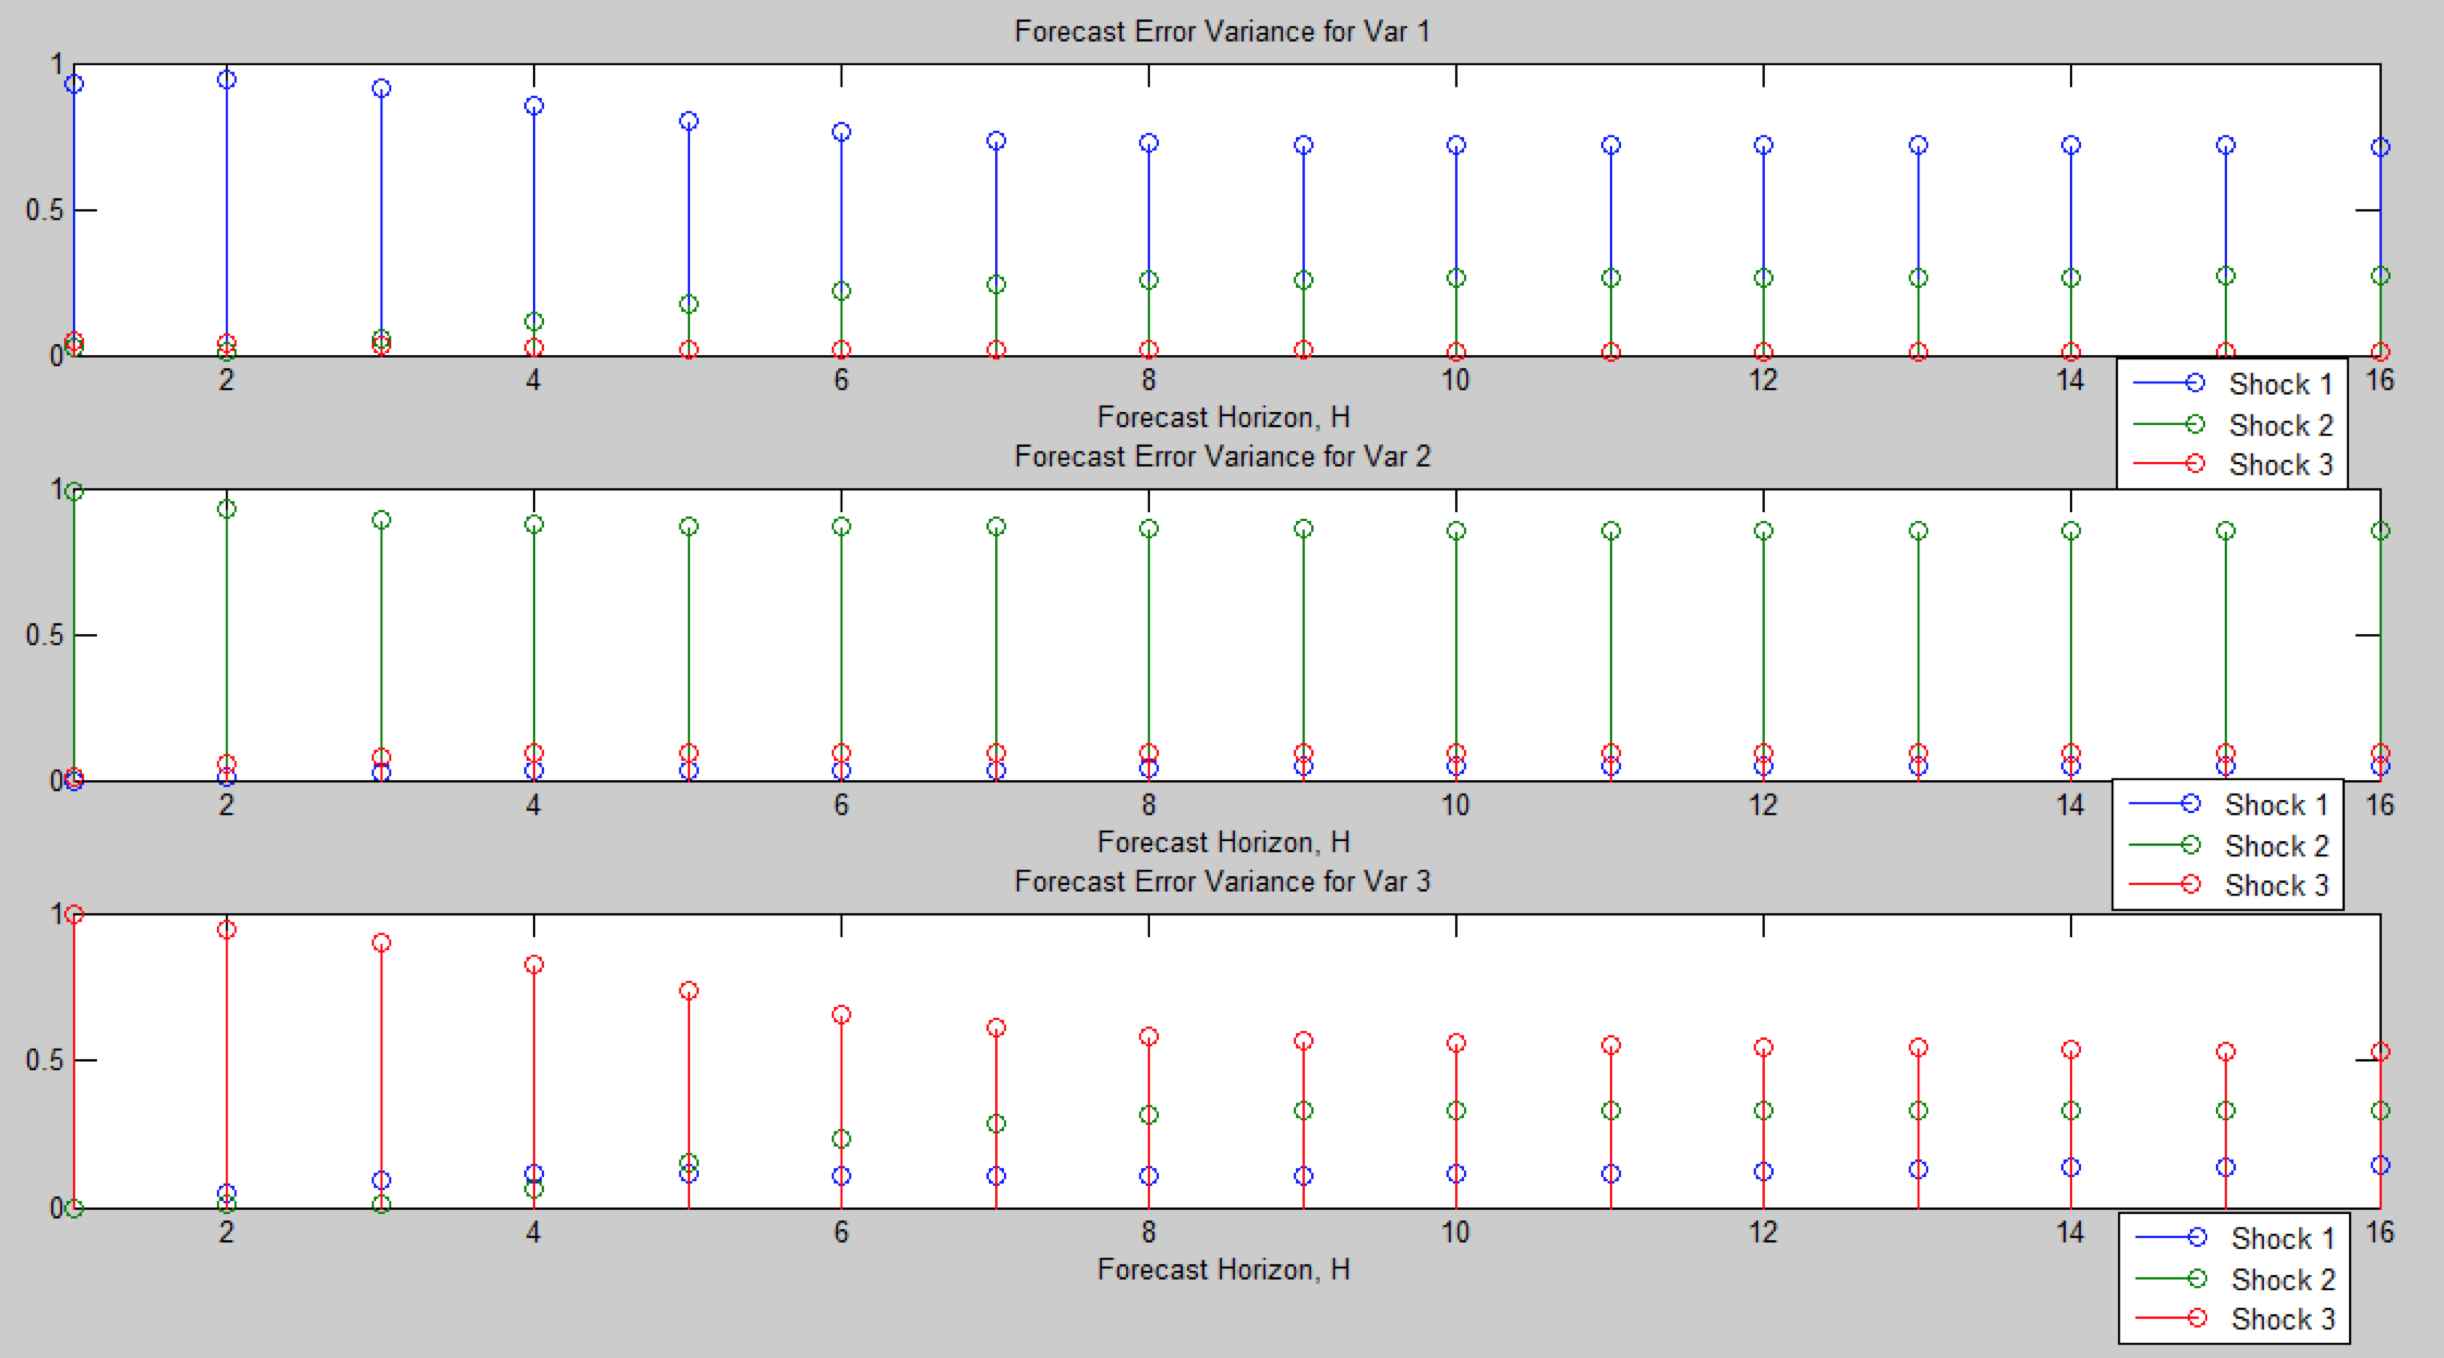
\includegraphics[scale=0.3]{forecast.png}
            \end{center}
            \par
            Carefully examining the above plots, we are able to figure out that the contribution of the interest rate to the forecast error variance diminishes over time and at some point becomes stable. The plot with respect to the growth rate shows an increasing trend in the first half and stablizing later. The contribution of the inflation rate is hardly visible in comparison. 
            \item The below are the IRF and the variance decompositions under the long-run restrictions.
            \begin{center}
            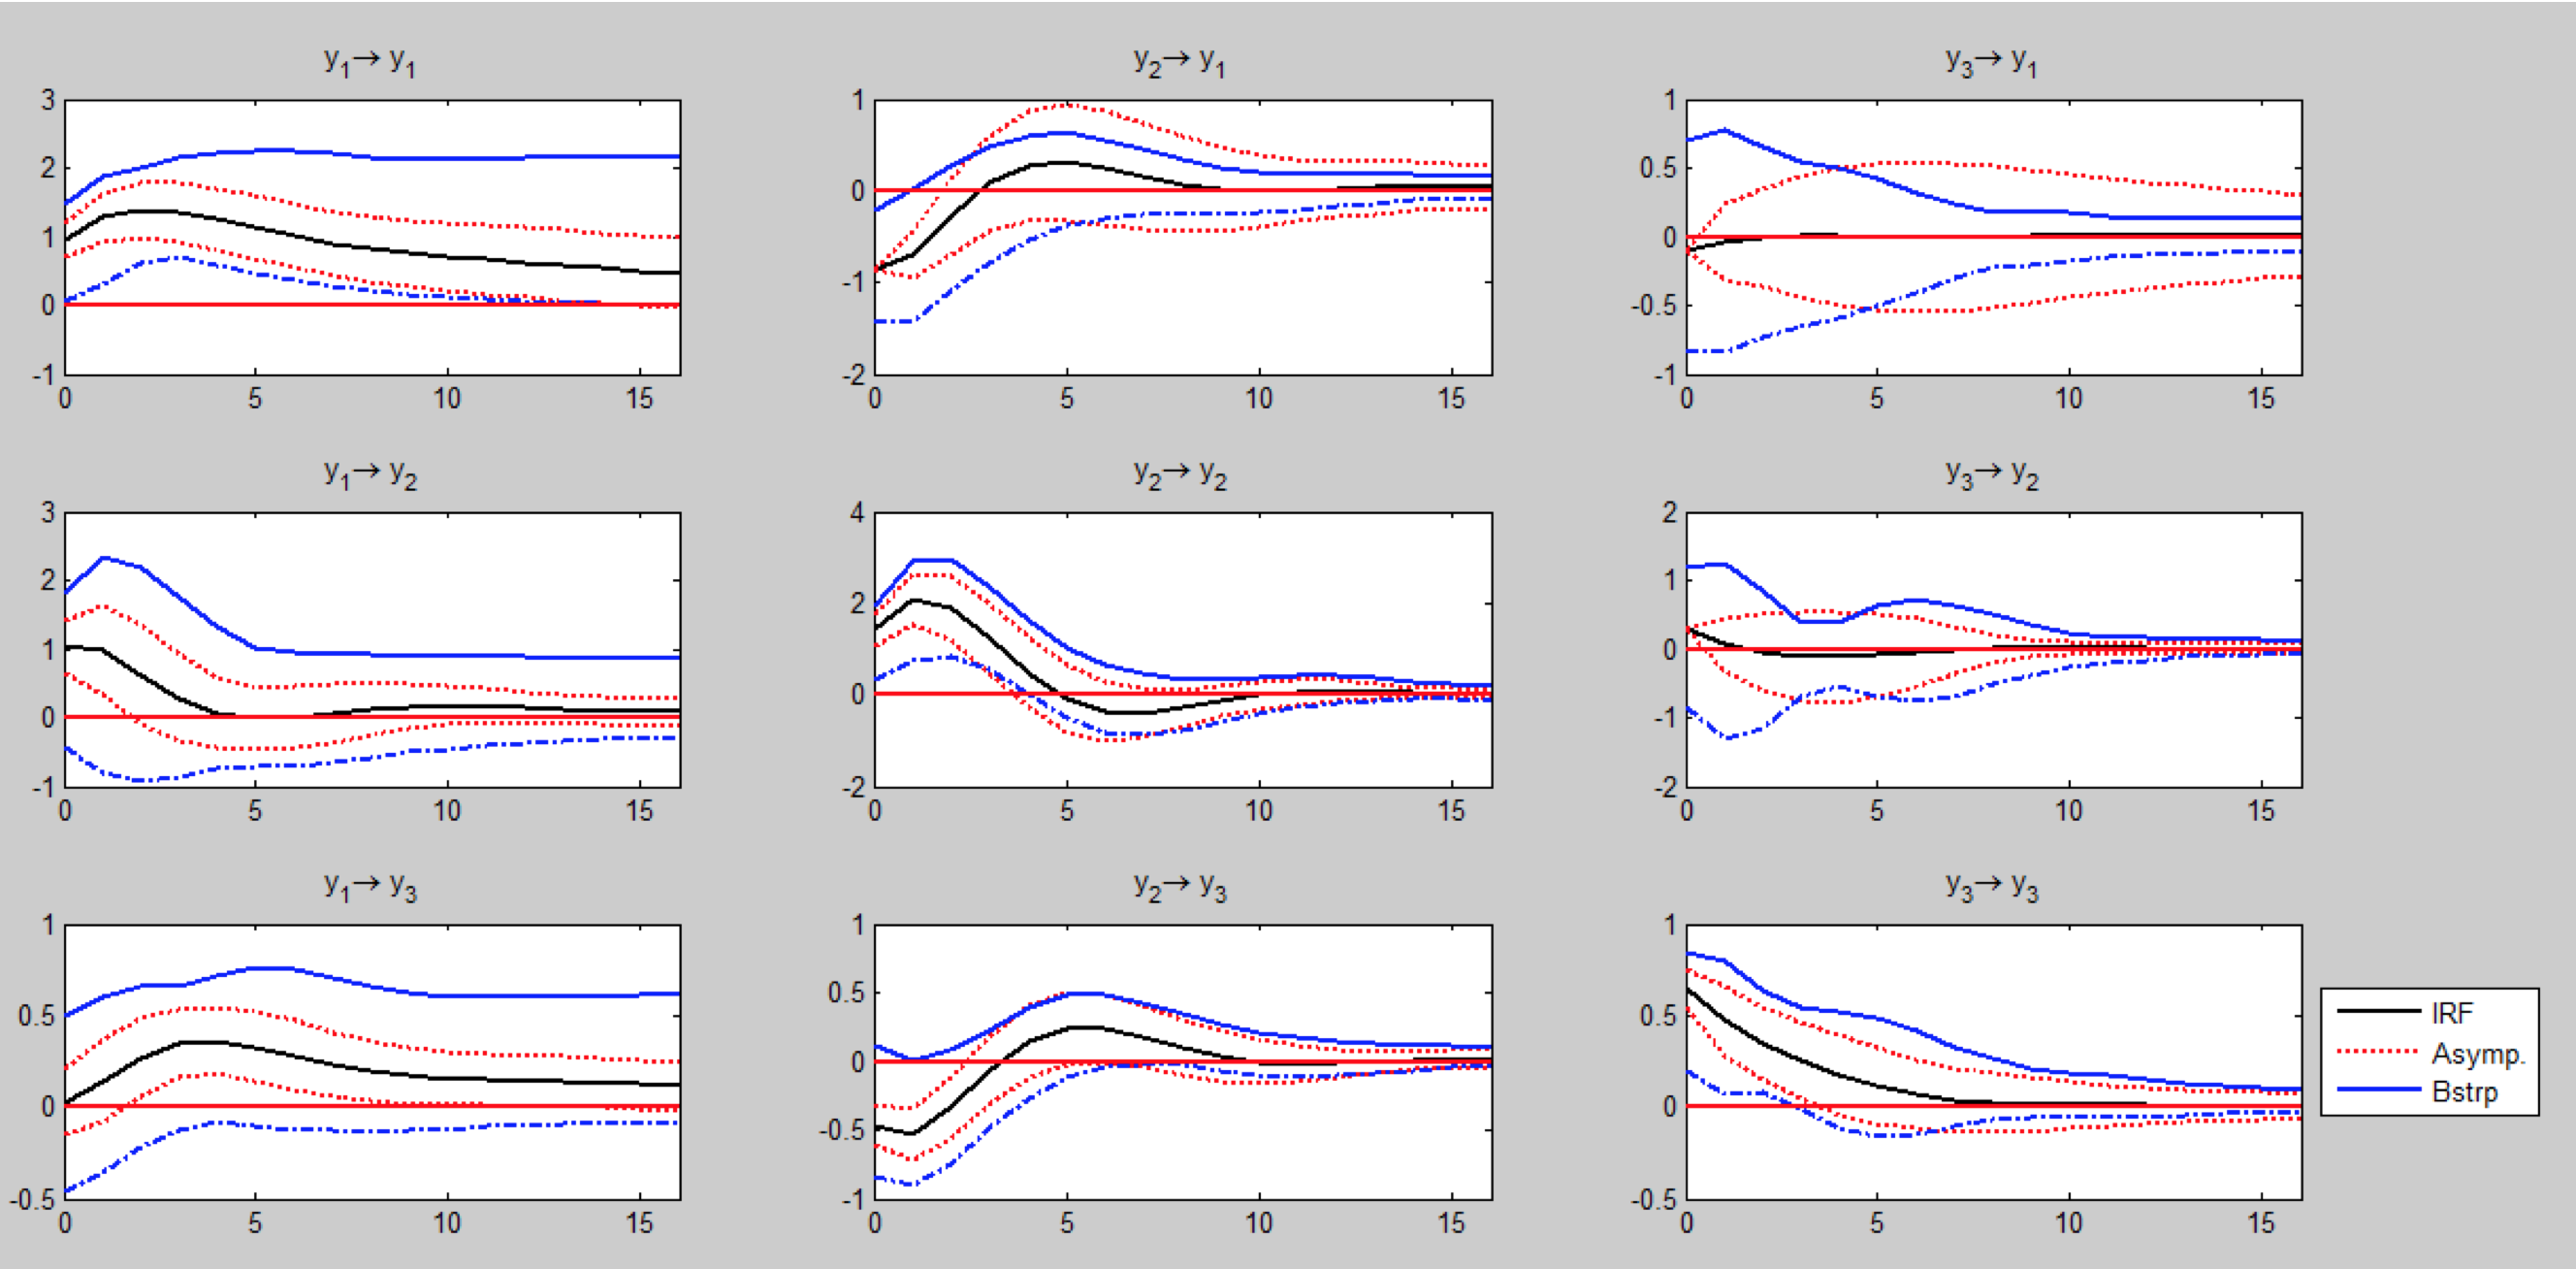
\includegraphics[scale=0.25]{IRF_long.png}
            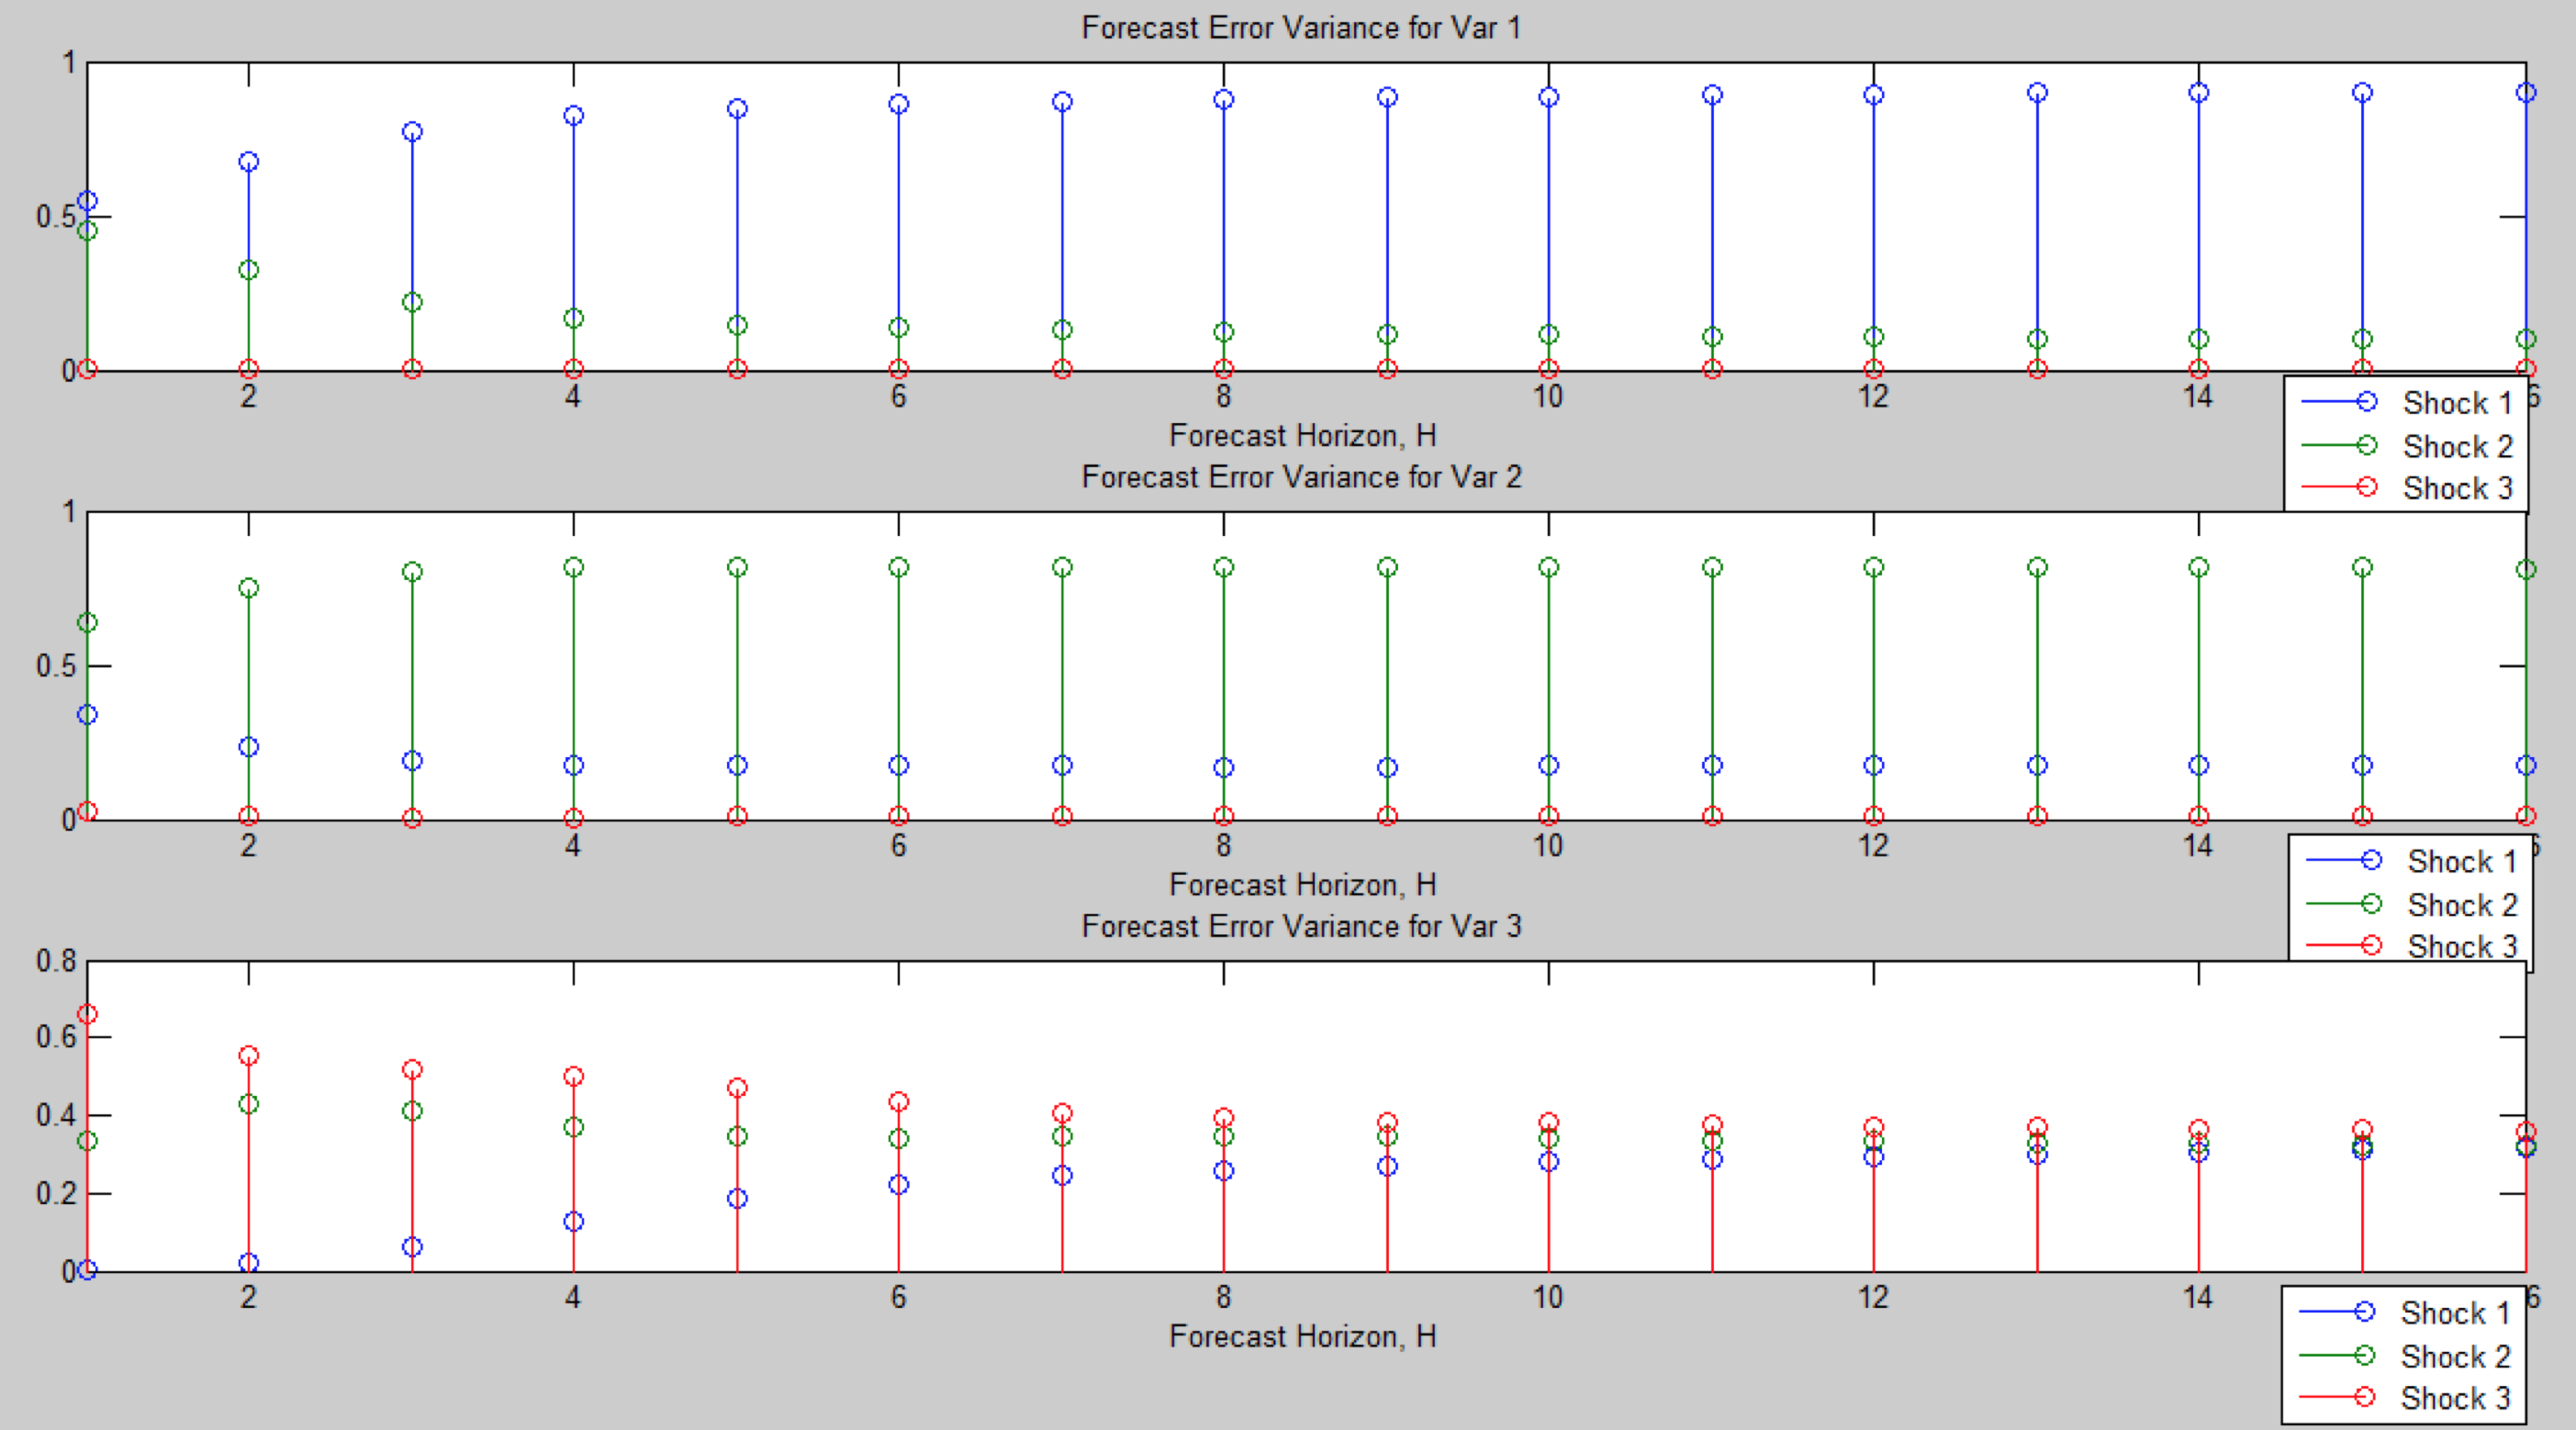
\includegraphics[scale=0.25]{vardecomp_long.png}
            \end{center}
            \par
            The IRF plots have changed except for the $(3,1)^{\text{th}}$ one and the diagonal plots. For the $(1,2)^{\text{th}}$ plot, it starts negative unlike the previous one although the overall shape hasn't changed much. The $(1,3)^{\text{th}}$ plot gives us the information that the interest rate is hardly ever affected by the inflation shock.
            \par
            The main difference of the first variable from the one under short-run restrictions is that the interest rate's contribution to the forecast error variance no longer decreases but rather increases and the growth rate's now decreases and does not increase. The second variable under the long-run restrictions has some influence on the interest rate. The third variable with respect to the growth rate shows decreasing influence and at some point later the three variables have equal contribution.
        \end{enumerate}
    \end{solution}
    \question
    Show that a vector autoregression is a special case of a seemingly unrelated regression.
    \begin{solution}
        For simplicity, consider VAR(1).
        \begin{align}
            y_{1t} &= \mu_{1}+a_{11}y_{1t-1}+a_{12}y_{2t-1}+u_{1t}\\
            y_{2t} &= \mu_{2}+a_{21}y_{1t-1}+a_{22}y_{2t-1}+u_{2t}
        \end{align}
        where $\operatorname{Cov}(u_{1t},u_{2t})=\sigma_{12}$ for $t=s$, $0$ otherwise. The model consists of 2 regression equations with different dependet variables but same independent variables. We could estimate the model using OLS estimator separately for each equation. This falls under the category of a seemingly unrelated regression where variables are contemporaneously correlated---which exactly means $\operatorname{Cov}(u_{1t},u_{2t})\neq 0$ for $t=s$---but uncorrelated over time---$\operatorname{Cov}(u_{1t},u_{2t})= 0$ otherwise. 
    \end{solution}
    \question
    Exercise \#3 on page 59 of the lecture note.
    \begin{solution}

    \end{solution}
\end{questions}
\end{document}
